\documentclass{article}
\usepackage[utf8]{inputenc}
\usepackage{datetime}
\usepackage{enumerate}
\usepackage{textcomp}
\usepackage{amsmath}
\usepackage[a4paper,margin=0cm,landscape]{geometry}
\usepackage{tikz}
\usetikzlibrary{positioning,shadows,arrows}

\title{\bf \Large ASSIGNMENT 1}
\author{Xinhao Luo}
\date{\today}

\def\math#1{$#1$}

\setlength{\textheight}{8.5in}
\setlength{\textwidth}{6.5in}
\setlength{\oddsidemargin}{0in}
\setlength{\evensidemargin}{0in}
\voffset0.1in

\begin{document}
\maketitle
\medskip

\clearpage

\section{Problem 1}

\begin{enumerate}[a)]
    \item All strings of 0's and 1's, with exactly one 0's at head and tail
    \item All strings of 0's and 1's
    \item All strings of 0's and 1's, with 0 at the third digit counting from the end
    \item All strings of 0's and 1's, with exactly three 1's
    \item All strings of 0's and 1's, with even number of 1's and 0's
\end{enumerate}

\clearpage

\section{Problem 2}

\begin{enumerate}[a)]
    \item Two leftmost conditions:
        \begin{enumerate}[1)]
        \item \math{S \xrightarrow{} 0S1S \xrightarrow{} 0\epsilon1S \xrightarrow{} 0\epsilon10S1S \xrightarrow{} 0\epsilon10\epsilon1S \xrightarrow{} 0\epsilon1\epsilon0\epsilon1 \xrightarrow{} 0101}
        \item  \math{S \xrightarrow{} 0S1S \xrightarrow{} 01S0S1S \xrightarrow{} 01\epsilon0S1S \xrightarrow{} 01\epsilon0\epsilon1S \xrightarrow{} 01\epsilon0\epsilon1\epsilon \xrightarrow{} 0101}
        \end{enumerate}
    \item \begin{enumerate}[1)]
        \item \math{S \xrightarrow{} 0S1S \xrightarrow{} 0S10S1S \xrightarrow{} 01S0S1\epsilon \xrightarrow{} 01S0\epsilon1\epsilon \xrightarrow{} 01\epsilon0\epsilon1\epsilon \xrightarrow{} 0101}
        \item \math{S \xrightarrow{} 0S1S \xrightarrow{} 0S1\epsilon \xrightarrow{} 01S0S1\epsilon \xrightarrow{} 01S0\epsilon1 \xrightarrow{} 01\epsilon0\epsilon1 \xrightarrow{} 0101}
    \end{enumerate}
    \item \begin{itemize}
                \item derivation a.1 and b.1
                    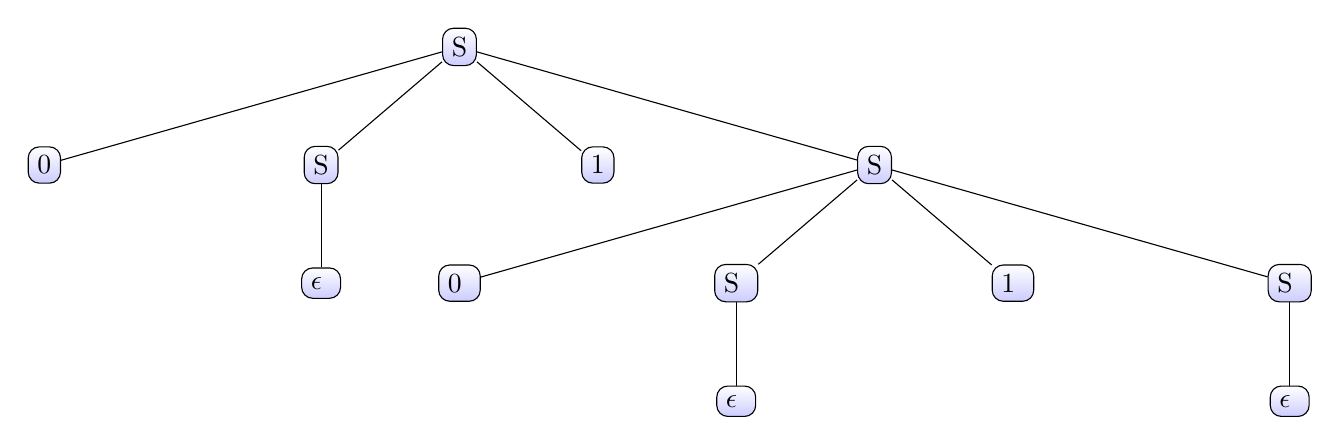
\begin{tikzpicture}[sibling distance=10em,
                      every node/.style = {shape=rectangle, rounded corners,
                        draw, align=center,
                        top color=white, bottom color=blue!20}]]
                      \node {S}
                        child { 
                            node{0}
                        }
                        child { node {S} 
                             child { node {\math{\epsilon} }} 
                             }
                        child { node {1} }
                        child { node {S} 
                            child { node { 0 } }
                            child { node { S }
                                child { node{\math{\epsilon} }}
                                }
                            child { node { 1 } }
                            child { node { S }
                                child { node{\math{\epsilon} }}
                                }
                        };
                    \end{tikzpicture}
                \item derivation a.2 and b.2
                    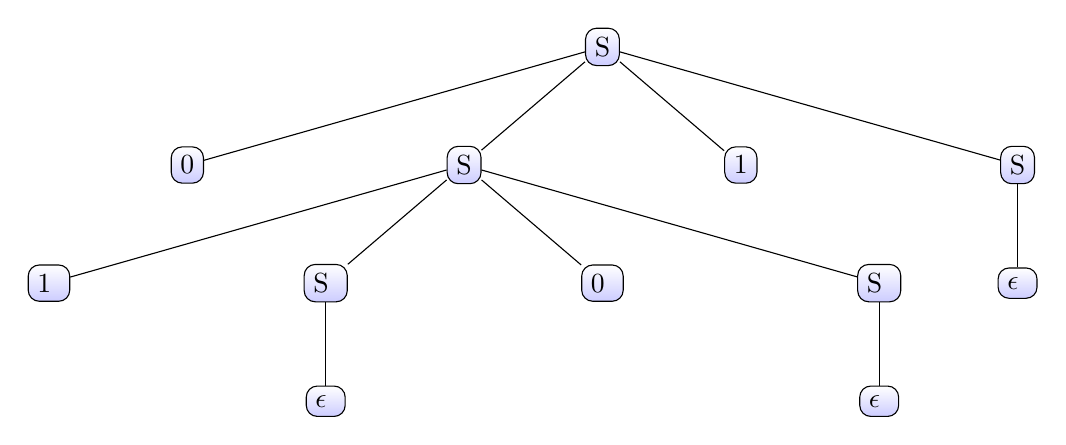
\begin{tikzpicture}[sibling distance=10em,
                      every node/.style = {shape=rectangle, rounded corners,
                        draw, align=center,
                        top color=white, bottom color=blue!20}]]
                      \node {S}
                        child { 
                            node{0}
                        }
                        child { node {S} 
                            child { node { 1 } }
                            child { node { S }
                                child { node{\math{\epsilon} }}
                                }
                            child { node { 0 } }
                            child { node { S }
                                child { node{\math{\epsilon} }}
                                }}
                        child { node {1} }
                        child { node {S}
                            child { node {\math{\epsilon} }} 
                        };
                    \end{tikzpicture}
        \end{itemize}
    \item Yes, there are 2 cases here. \\ 
    Assume we have a string x where count1(x) = count0(x), if the x start with 0, we may have x = 0y, where count1(y) = count0(y) + 1. Based on y, we may also have a 1 inside, which has a form y = a1b. Here we have count1(0a1b) = count0(0a1b), where a and b are string with same number of 1 and 0. So we have every string with equal number of 0's and 1's and started with 0 can be written in form 0a1b, which is corresponded to \math{S \xrightarrow{} 0S1S}. \\
    Similar procedures can applied to string started with 1 and we may have 1a0b, which is corresponded to \math{S \xrightarrow{} 1S0S}. \\
    The grammar covered both cases so all string with equal number of 0's and 1's can be generated from this grammar.
\end{enumerate}

\clearpage

\section{Problem 3}
\begin{enumerate}[a)]
    \item Given string: id \math{\theta_{n}} id \math{\theta_{n}} id , two different parse tree can be generated, which prove the grammar is a ambiguous 
        \begin{enumerate}[1)]
            \item 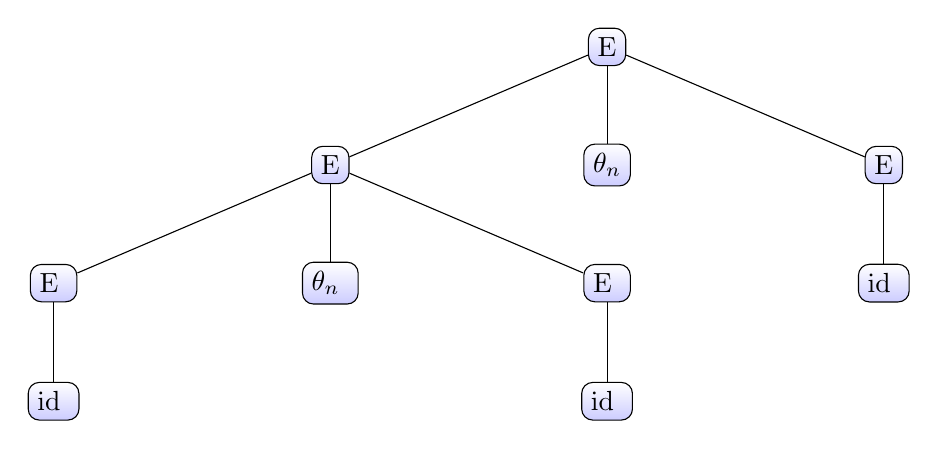
\begin{tikzpicture}[sibling distance=10em,
                      every node/.style = {shape=rectangle, rounded corners,
                        draw, align=center,
                        top color=white, bottom color=blue!20}]]
                      \node {E}
                        child { node {E} 
                            child { node { E }
                                child { node{ id }}
                                }
                            child { node { \math{\theta_{n}} } }
                            child { node { E }
                                child { node{ id }}
                                }}
                        child { node {\math{\theta_{n}}} }
                        child { node {E}
                            child { node { id }} 
                        };
                    \end{tikzpicture}
                \item 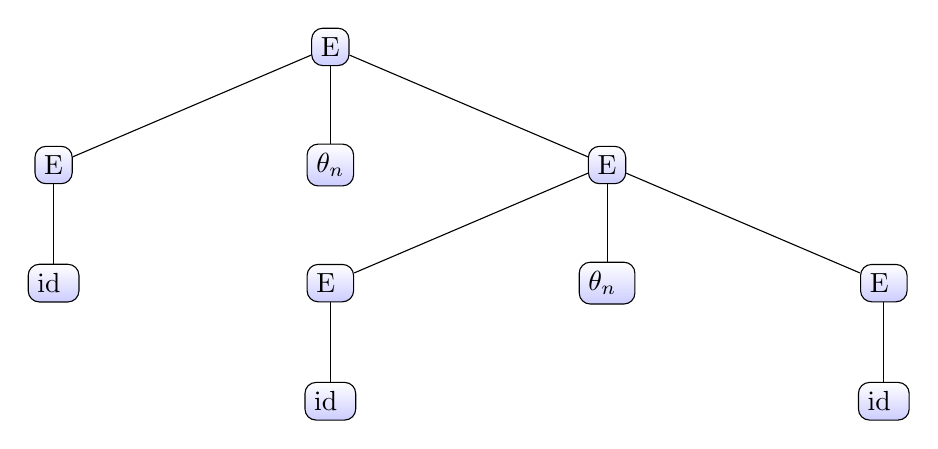
\begin{tikzpicture}[sibling distance=10em,
                      every node/.style = {shape=rectangle, rounded corners,
                        draw, align=center,
                        top color=white, bottom color=blue!20}]]
                      \node {E}
                        child { node {E}
                            child { node { id }} 
                        }
                        child { node {\math{\theta_{n}}} }
                        child { node {E} 
                            child { node { E }
                                child { node{ id } }
                            }
                            child { node { \math{\theta_{n}} } }
                            child { node { E }
                                child { node{ id }}
                                }};
                    \end{tikzpicture}
        \end{enumerate}
    \item \begin{equation}
        \begin{split}
             E &\xrightarrow{} {Terms}_{1} \theta_{1} E | {Terms}_{1} \\
             {Terms}_{1} &\xrightarrow{} {Terms}_{2} \theta_{2} {Term}_{1} | {Terms}_{2} \\
             {Terms}_{2} &\xrightarrow{} {Terms}_{3} \theta_{3} {Terms}_{2} | {Terms}_{3} \\
              &... \\
             {Terms}_{n-1} &\xrightarrow{} {Terms}_{n} \theta_{n} {Terms}_{n - 1} | Terms_{n} \\
             {Terms}_{n} &\xrightarrow{} {Terms}^{*} | Terms \\
             {Terms} &\xrightarrow{} id | (E)
        \end{split}
    \end{equation}
\end{enumerate}

\clearpage

\section{Problem 4}
\begin{enumerate}[a)]
    \item \begin{itemize}
        \item FOLLOW(\math{Es}) = \{\texttt{)}\}
    \item FOLLOW(\math{E}) = \{ \texttt{(}, \texttt{)}, \texttt{\$\$}, \texttt{atom}, \texttt{'} \}
    \item PREDICT(\math{Es \xleftarrow{} \epsilon}) = \{\texttt{)}\}
    \end{itemize}
    \item 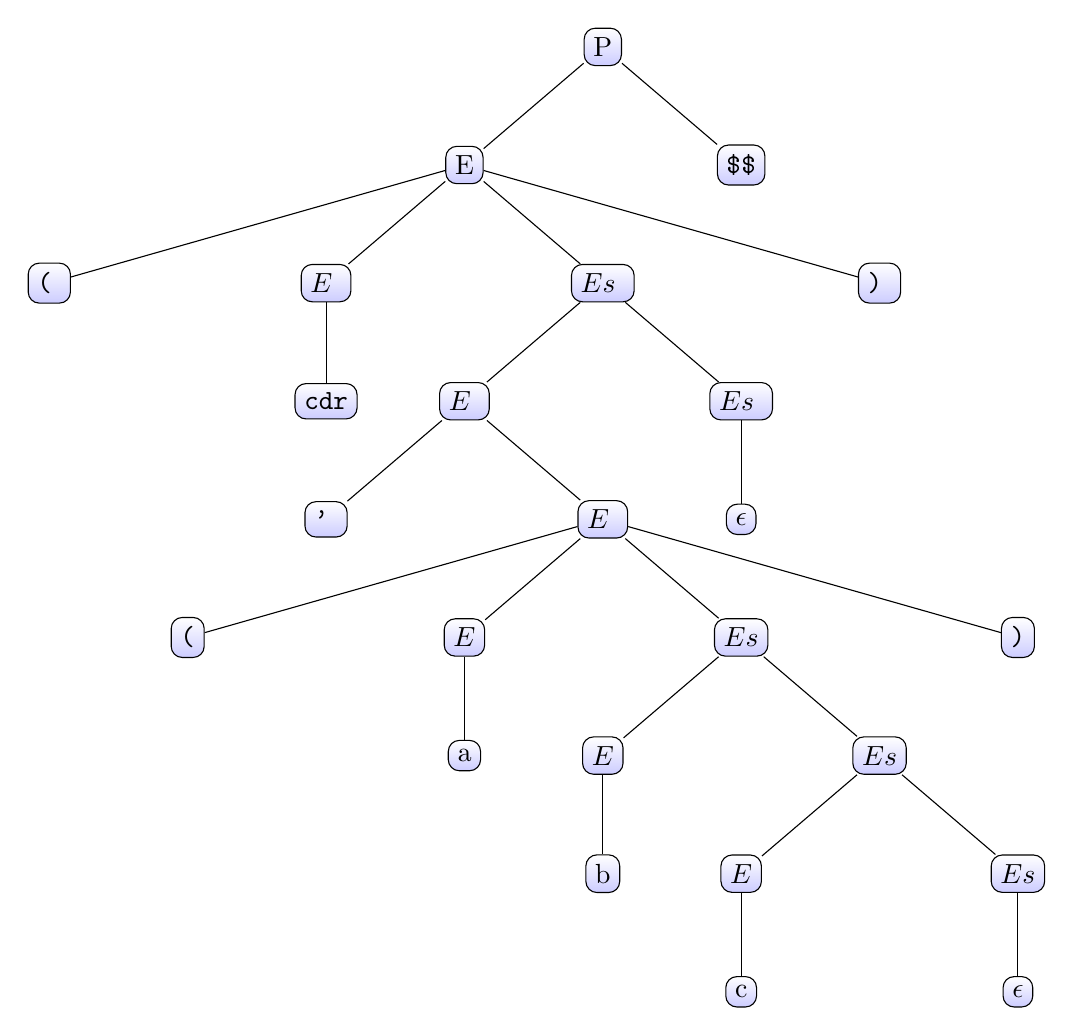
\begin{tikzpicture}[sibling distance=10em,
                      every node/.style = {shape=rectangle, rounded corners,
                        draw, align=center,
                        top color=white, bottom color=blue!20}]]
                      \node {P}
                        child { node {E} 
                            child { node { \texttt{(} } }
                            child { node { \math{E} } 
                                child { node { \texttt{cdr}} }
                                }
                            child { node { \math{Es} }
                                child { node{ \math{E} }
                                    child {
                                        node { \texttt{'} }
                                    }
                                    child {
                                        node { \math{E} }
                                        child { node {\texttt{(}} }
                                        child { node {\math{E}}
                                            child { node {a} }
                                        }
                                        child { node {\math{Es}} 
                                            child { node {\math{E}} 
                                                child { node {b} }
                                            }
                                            child { node {\math{Es}} 
                                                child { node {\math{E}} 
                                                    child { node {c} }
                                                }
                                                child { node {\math{Es}} 
                                                    child { node {\math{\epsilon}} }
                                                }
                                            }
                                        }
                                        child { node {\texttt{)}} }
                                    }
                                }
                                child { node{ \math{Es} }
                                        child { node {\math{\epsilon}} }
                                    }
                                }
                            child { node { \texttt{)} }}    
                            }
                        child { node {\texttt{\$\$}} };
                    \end{tikzpicture}
    \item Active Routines: (stack should be the left side of the productions)
        \begin{equation}
            \begin{split}
                P &\xrightarrow{} E\$\$ \\
                E &\xrightarrow{} (EEs)\\
                Es &\xrightarrow{} E Es \\
                E &\xrightarrow{} \texttt{'}E 
            \end{split}
        \end{equation}
\end{enumerate}


\clearpage

\section{Problem 5}

\begin{enumerate}[1)]
    \item Ambiguous: NO, LL(1): No
    \item Ambiguous: NO, LL(1): Yes
    \item Ambiguous: YES, LL(1): No % ()() 有两种
    \item Ambiguous: YES, LL(1): No
    \item Ambiguous: NO, LL(1): Yes
\end{enumerate}

\end{document}
